\chapter{Global Supercoiling in \emph{Aevol}}
\label{chap:aevol}

In this chapter, I present the first main line of work of that I undertook during my Ph. D., in which I implemented a model of the effect of DNA supercoiling on gene transcription into the \emph{Aevol} \emph{in silico} experimental evolution platform, in order to study the possible epistatic interactions between mutations that regulate the supercoiling level and other kinds of mutations.

\section{Introduction}
\label{sec:aevol:intro}

In the \emph{Long-Term Evolution Experiment}, started by Richard Lenski in 1988~\citep{lenski1991}, 12 populations of \emph{E. coli}, originating from the same ancestral strain, were placed to evolve in a new environment, a glucose-limited medium.
Every day since the beginning of the experiment, which is still running, a sample from each population has been propagated into fresh medium, resulting in the longest-running evolution experiment in the lab, and demonstrated that fitness can keep on increasing for much longer than originally expected in a constant environment~\citep{good2017}.
As sequencing capacity and synthetic biology developed in the late 1990s and early 2000s, identifying the precise DNA mutations underpinning these increases in fitness became possible.
Mutations in the \emph{fis} and \emph{topA} gene were thus found to lead to an increased growth rate in the conditions of the experiment, as well as to an increase in the basal supercoiling level of the cells bearing these mutations~\citep{crozat2005}.
\textbf{Devrait plutôt aller dans l'intro globale ?
Tel quel ça pose la question du rôle de la superhélicité dans l'évolution mais il n'y a pas (dans Crozat 2005 ou 2010) d'étude des suites évolutives de ces mutations de superhélicité.}

As mutations in genes regulating the level of supercoiling in \emph{E. coli}, such as \emph{topA} and \emph{fis}, were shown to increase fitness in the LTEE, we sought to investigate whether these mutations, by globally altering the regulatory landscape of the cell, could open up new evolutionary pathways and thereby speed up evolution, that is display positive epistasis with other mutations.
In order to explore this theoretical possibility without having to resort to wet-lab experiments, I resorted to the \emph{in silico} experimental evolution toolbox, using the \emph{Aevol} platform.


\section{The \emph{Aevol} model}
\label{sec:aevol:model}

\begin{figure}[H]
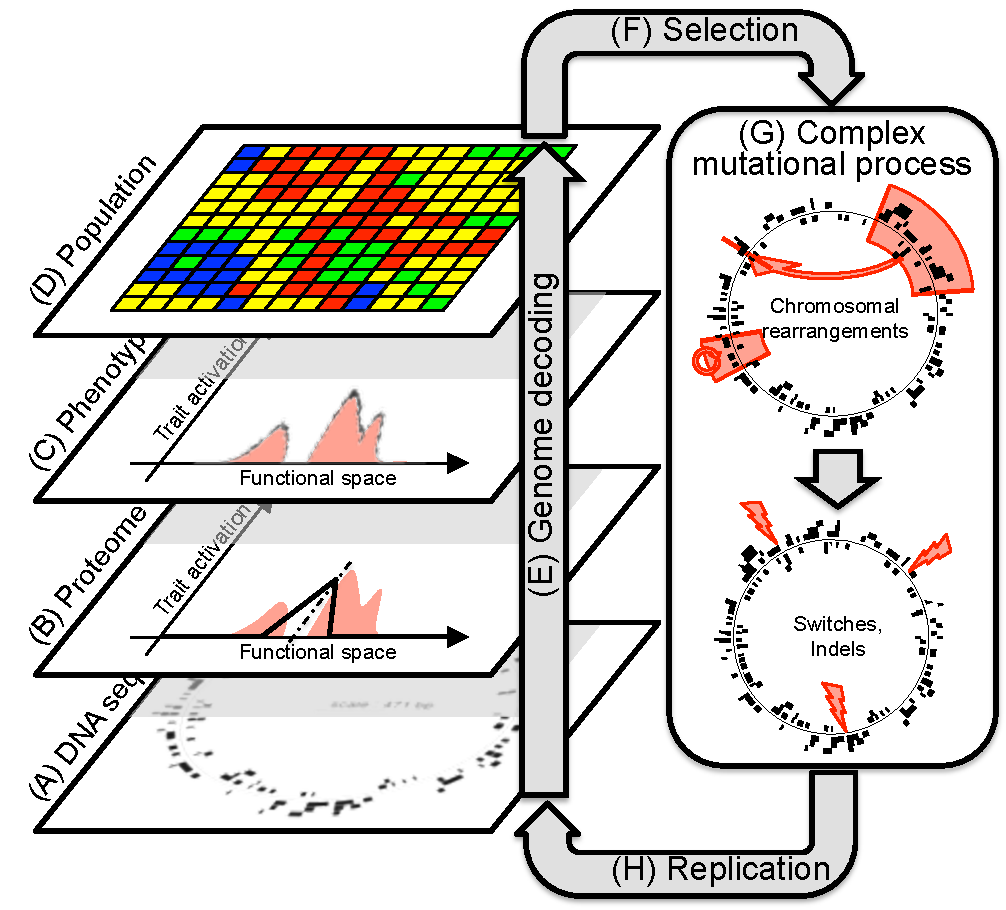
\includegraphics[width=\textwidth]{aevol/images/aevol.pdf}
\caption[Overview of the \emph{Aevol} model]{Broad overview of the \emph{Aevol} model.}
\label{fig:aevol:model}
\end{figure}

\subsection{Overview}

The \emph{Aevol} platform, developed in the Inria Beagle team~\citep{rutten2019}, is a software suite designed to run artificial evolution experiments on a computer, rather than at the bench.
As an excellent and very thorough description of \emph{Aevol} (in French) can be found in~\cite{liard2020b}, the following presentation of the model will be kept short and to the point.
Figure~\ref{fig:aevol:model} provides a comprehensive overview of the evolutionary algorithm at the core of \emph{Aevol}.
It follows the evolution over a given number of discrete generations of a population of individuals that are defined by their genome, encoded as a circular string of nucleotides (A), in an environment described by a phenotype that is optimal in this environment.
At every generation, the genome of every individual is transcribed into RNA then translated into proteins (B), following the ``central dogma of molecular biology''~\citep{crick1958}.
These proteins are then mapped to an abstract phenotypic space (C), and the resulting phenotype is compared to the optimal phenotype in order to compute the fitness of the individual.
The population is laid out on a square grid (D), with one individual per cell.
In order to produce a new generation, the ancestor of the new individual in each cell is chosen at random among the neighboring individuals, proportionally to their fitness (F).
Once this ancestor is chosen, its genome undergoes a series of random mutations, including genomic rearrangements as well as local mutations (G), in order to obtain the genome of the new individual in the cell at the next generation (H).

\subsection{The Genotype-Phenotype Map in \emph{Aevol}}

A genome in \emph{Aevol} consists in a sequence of binary characters ($0$ or $1$), representing a double-stranded circular sequence of DNA.
The genome sequence explicitly describes the first (leading) strand, while the second (lagging) strand is obtained by taking the complement of the sequence, replacing $0$ by $1$ and vice-versa.
The decoding algorithm starts by looking for sequences that code for RNAs, reading the leading strand left-to-right and the lagging strand right-to-left.
An RNA starts with a promoter sequence, which has to match a consensus sequence up to $d_{max}$ errors, and ends with a hairpin-like terminator.
Then, each RNA is scanned for genes, which start with a ribosome binding site followed by a 3-nucleotide start codon.
Reading continues until a stop codon is found in the same frame, and the resulting string of codons is then translated into a protein, or discarded if there no stop codon was found before the end of the RNA sequence.
An RNA can thus contain zero, one, or several protein-coding genes.

As the genetic alphabet is binary in \emph{Aevol}, there are 8 different 3-nucleotide codons, and 6 codons can therefore be used to encode protein data, on top of the start and stop codons.
These codons are grouped into three pairs, each respectively encoding the width $w$, height $h$, and mean position $m$ of a kernel function from $[0, 1]$ to $[0, 1]$.
The mean $m$ represents the main function that the protein fulfills in the abstract phenotypic space, the height $h$ the intensity with which it does, and the width $w$ the pleiotropic ability of the protein to fulfill neighboring phenotypic functions.

In order to obtain the final contribution of the protein to the phenotype, the constitutive height $h$ of the gene is weighted by the expression level $e$ of the RNA that carries it.
This expression level depends on the difference $d$ between the promoter sequence of this RNA and the consensus sequence: $e = 1 - \frac{d}{1+d_{max}}$.
Finally, in order to compute the complete phenotype of the individual from the set of its proteins, the kernel functions representing each gene are summed, resulting in a piecewise-linear phenotype function.
As the maximum degree to which each phenotypic function can be fulfilled is bound to 1, the phenotype function is finally capped using Łukasiewicz operators in order to keep within this limit.

\subsection{Fitness}

Once the phenotype of an individual has been decoded from its genome, we can compute its fitness.
As the environment is specified using an optimal phenotype, we first compute a gap value as the integral of the absolute value of the difference between the phenotype of the individual and the optimal phenotype, taken over the range of phenotypic values (the $L^1$ distance between the functions).
Then, we compute the fitness as the inverse exponential of the gap, multiplied by a selection coefficient: the higher the coefficient, the larger the difference in fitness between individuals with the same difference in gap.

\subsection{Mutational Operators}

Once the ancestor of a new individual has been chosen, a set of random mutations are applied to its genome to obtain the new genome.
These mutations are split in two classes, depending on the proportion of the genome that they can affect.
Genomic rearrangements, which can change up to the whole genome, comprise large-scale deletions and duplications, inversions, and translocations.
Local mutations, on the contrary, comprise small insertions, small  deletions (collectively known as indels), and switches.

\subsection{Modeling DNA Supercoiling in \emph{Aevol}}

In order to model the effect of supercoiling on gene transcription in \emph{Aevol}, I chose to start with a very simple approximation, considering that the supercoiling level is constant along the genome and over time.
This can be interpreted as considering the spatial and temporal average of the (actually dynamic) supercoiling level.
To implement this model inside \emph{Aevol}, I changed the genotype of individuals by adding, alongside the string-of-nucleotide genome, a single parameter $\gamma$, which represents the variation in the supercoiling level $\sigma$ of this individual compared to a reference supercoiling level $\sigma_0$: $\gamma = \frac{\sigma-\sigma_0}{\sigma_0}$.

\paragraph{Gene Expression}
To keep the model as simple as possible, I also chose to model the effect of supercoiling on transcription as linear for all genes, updating the computation of the final expression level $e$ to take supercoiling into account:

\begin{equation}
e = (1 - \frac{d}{1+d_{max}}) \cdot (1 - \gamma)
\label{eq:aevol:sc}
\end{equation}

When $\gamma$ is equal to 0, the supercoiling level is equal to the baseline, resulting in no change to the expression level.
When $\gamma < 0$, that is when supercoiling is negative, gene expression is increased; and when $\gamma > 0$, gene expression is decreased.
Note that, when keeping $\gamma$ to 0, the behavior of the vanilla \emph{Aevol} model is replicated in this model.

\paragraph{Mutational Operator}
In real organisms, the supercoiling level is not a direct property of the genome but is controlled by a set of proteins that are not modeled in \emph{Aevol} (as the phenotypic space is completely abstract), and changes in the supercoiling level come from mutations affecting these proteins.
In order to model mutations in the supercoiling level in \emph{Aevol}, I therefore chose a continuous variation model, which directly reflects the effect of the mutation in the supercoiling-controlling genes.
When an individual reproduces, we first use a Bernoulli trial with a probability $p$ that represents the probability of a supercoiling-protein gene to undergo a non-synonymous mutation, and change the supercoiling level, during reproduction.
Then, if the supercoiling level changes, we pick the variation in relative supercoiling $\delta\gamma$ according to a normal distribution $\mathcal{N}(0, s^2)$, and finally set the relative supercoiling level $\gamma'$ of the offspring to $\gamma' = \gamma + \delta\gamma$.
The parameters of these laws are given as parameters to the simulation, and their values are given in Table~\ref{tab:aevol:param_values}.
Throughout this chapter, I will for clarity refer to the usual DNA-affecting mutations presented in~\ref{sec:aevol:model} as \emph{genomic mutations}, and to mutations in the supercoiling level as \emph{supercoiling mutations}.


\section{Results}
\label{sec:aevol:results}

The goal of implementing a supercoiling model in \emph{Aevol} was twofold.
The first aim was to see to which extent adding a new dimension to the phenotypic space, and a new mutational operator to explore it, would allow for faster adaptation than allowed by the original model, thank to the wide jumps in the phenotypic landscape made possible by these mutations.
The second aim was to disentangle the possible epistatic effects between supercoiling mutations and genomic mutations in \emph{Aevol}.
In this section, I first present the experimental setup that I used in order to answer these questions.
Then, I show that adding regulation by supercoiling did not measurably increase the rate of adaptation of the populations compared to the control, and that supercoiling indeed follows a very constrained evolutionary trajectory in these experiments.
Finally, I conclude that I could not find any observable epistasis between supercoiling and other mutations, when using the supercoiling model presented in Section~\ref{sec:aevol:model}.

\subsection{Experimental Setup}

In order to tackle these questions, I ran two sets of simulations: the experimental runs using the supercoiling model, and the control runs using the vanilla version of \emph{Aevol}.
Each set of runs comprises 5 replicate populations, which evolved for 1,000,000 generations, starting from a clonal population.
The initial individual was obtained for each run by randomly drawing 5,000 bp-long genomes, until a genome with a non-zero fitness (i.e., at least one protein-coding gene partially matching the phenotypic target) was found.
The simulations were run on a 24-core Intel(R) Xeon(R) CPU E5-2620 v3 @ 2.40GHz server with 128 GB of RAM, and lasted approximately a week for each set of replicates.
I simulated the evolution of only a limited number of replicates with and without supercoiling, out of concern for the energy expenditure of the simulations as the work was preliminary.


\paragraph{Studying Lineages}
The data that is presented in the rest of this section was obtained by reconstructing the lineage, starting from the initial generation, of a random individual at the last generation of each replicate.
Studying a given lineage, rather than the best individual at every generation (which need not sire one another), allows us to reconstruct the precise set of mutations that happened throughout the evolutionary history of this lineage, and therefore gives us information about the possible causal link between these mutations.

As a theoretical haploid Wright-Fisher population with $N$ individuals coalesces on average in $2N$ generations (without selection) (\textbf{citation ? dans Felsenstein}), we chose to analyze the data from generation 0 to 990,000 (taking out the last 10,000 generations), ensuring that this lineage is indeed ancestral to the whole population of the last generation.

\begin{table}[h]
  \begin{center}
    \begin{tabular}{ l r r }
    \toprule
    \textbf{Parameter} & \textbf{Symbol} & \textbf{Value}\\
    \midrule
    Population size & N & 1,024 (32x32 grid) \\
    Initial genome size & $g_0$ & 5,000 bp \\
    Local mutation rate & $\mu_{loc}$ & $10^{-7}$ bp$^{-1}$.gen$^{-1}$ \\
    Rearrangement rate & $\mu_{rear}$ &$10^{-6}$ bp$^{-1}$.gen$^{-1}$ \\
    \midrule
    Initial supercoiling level & $\gamma_0$ & 0 \\
    Supercoiling mutation probability & $p$ & $10^{-1}$ \\
    Supercoiling mutation variance & $s^2$ & $10^{-2}$ \\
    \midrule
    Generations & T & 1,000,000 \\
    Replicates & $n$ & 5\\
    \bottomrule
    \end{tabular}
    \end{center}
  \caption[Table of parameter values for the \emph{Aevol} runs]{Table of parameter values used in the \emph{Aevol} evolutionary runs.
  The top part describes parameters common to the experimental and control set of rules, the middle part the supercoiling-related parameters introduced in the supercoiling model, and the bottom part the simulation parameters.}
  \label{tab:aevol:param_values}
\end{table}

\subsection{Evolution of the Fitness Level}

\begin{figure}[H]
  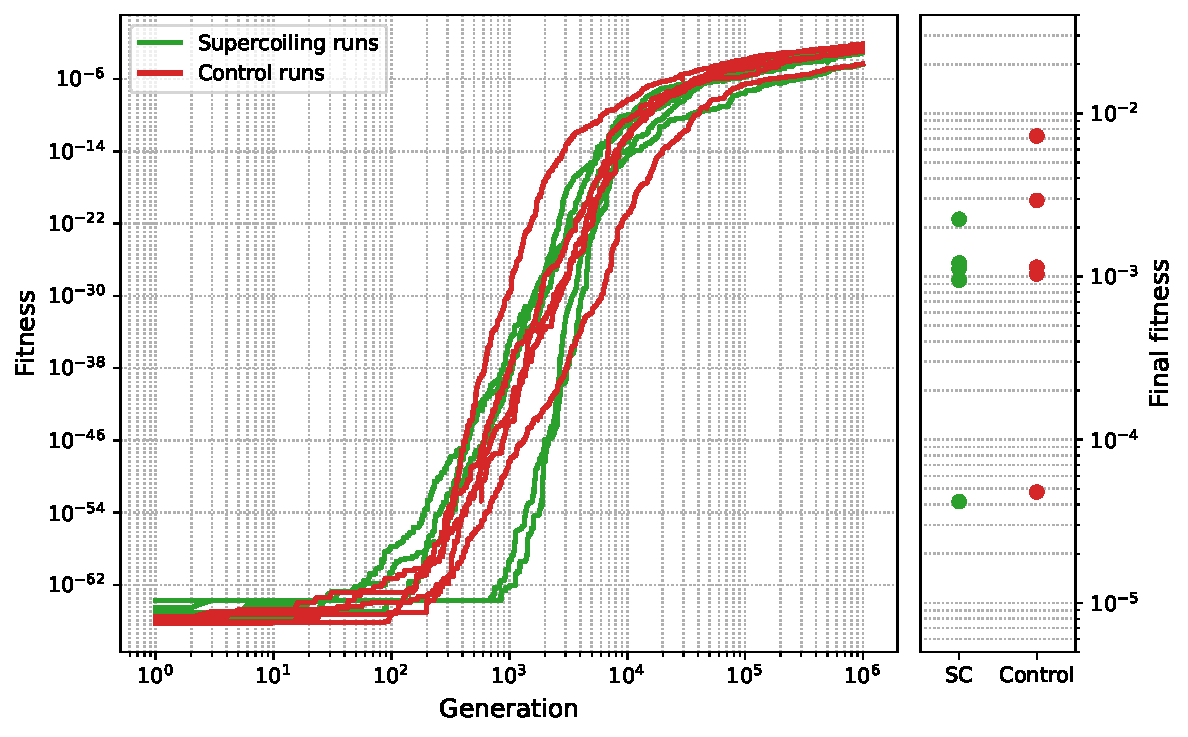
\includegraphics[width=\textwidth]{aevol/images/fitness_all.pdf}
  \caption[Evolution of the fitness of the control and experimental runs in \emph{Aevol}]{Left: Evolution of the fitness at every generation throughout the lineage of the final population of each replicate of the experimental (green) and control (red) runs.
  Both axes follow logarithmic scales.
  Right: Fitness of the lineage individual at the 990,000th generation of each run, separated between supercoiling (green) and control (red) runs.}
  \label{fig:aevol:fitness}
\end{figure}

Figure~\ref{fig:aevol:fitness} presents, on the left-hand side, the fitness of the individual at every generation of the lineage of the final population, in each replicate.
In each case, the fitness follows a broadly sigmoid shape, quickly increasing during the first 100,000 generations of the run, then slowing down for the remaining 900,000 generations, but never completely ceasing to increase.
The right-hand side of Figure~\ref{fig:aevol:fitness} shows the fitness of the lineage individual at the 990,000th generation.

Even with the limited number of replicates of each run, there is no discernible difference in fitness between the two experimental conditions, with and without mutations in the supercoiling level.
Adding the new phenotypic dimension of the supercoiling level, and the associated supercoiling mutational operator, therefore did not seem to play an important role in the evolution of populations in \emph{Aevol}.

\subsection{Evolution of the Supercoiling Level}

\begin{figure}[H]
  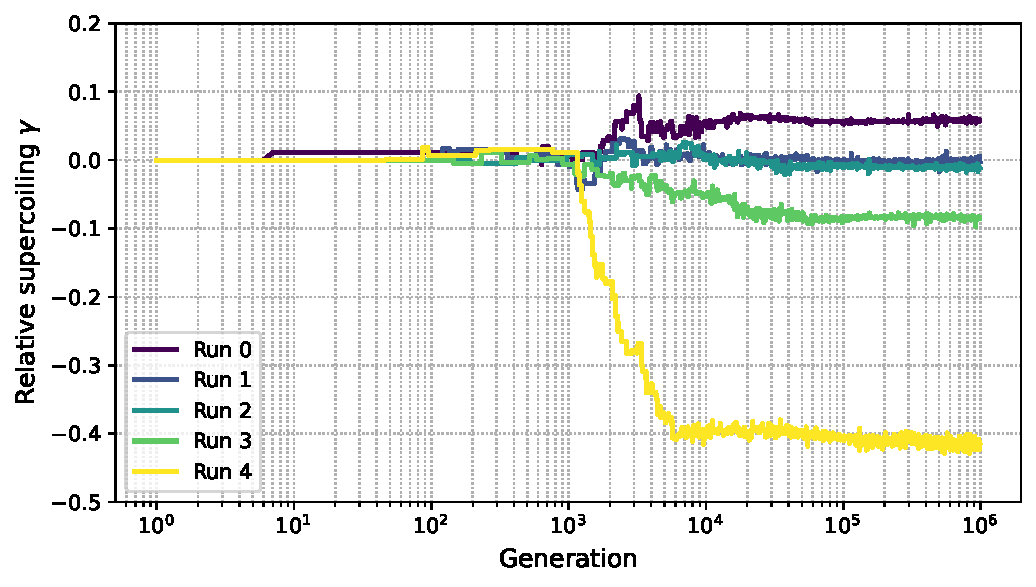
\includegraphics[width=\textwidth]{aevol/images/supercoiling_all.pdf}
  \caption[Evolution of the supercoiling level of the experimental runs in \emph{Aevol}]{Evolution of the relative level of supercoiling at every generation of the lineage of each of the experimental runs.}
  \label{fig:aevol:sc}
\end{figure}

Figure~\ref{fig:aevol:sc} shows the evolution of the supercoiling level throughout the lineage in each of the 5 replicates.
In every run, the supercoiling level evolves only at the very beginning of the run, stabilizing in a few tens of thousands of generations, and remaining essentially constant afterwards.
This is in strong contrast to the fitness of the runs (presented in Figure~\ref{fig:aevol:sc}), which keeps increasing until the end of the runs.

It therefore seems that the supercoiling level might play a role in the early evolution of the runs, but not in their long-term fitness improvement.
This result can be disappointing but was not entirely unexpected.
Indeed, in the early evolution of individuals in \emph{Aevol}, the phenotypic target is only very imperfectly fit by the proteins expressed by the individual.
At that stage, mutations in the supercoiling level, which affect the expression level of every protein equally, could indeed be favorable by bringing the whole phenotype closer to the optimum, in a very broad swipe.
More precisely, at the early stage of evolution in \emph{Aevol}, phenotypic functions are often under-performed by individuals, as the width of the kernel functions can be small, or the expression level of the RNAs low if the promoter contains many errors.
At that stage, an increase in negative supercoiling could be adaptive, as it boosts gene expression levels.
This could explain why run 4 in the simulations (Figure~\ref{fig:aevol:sc}, in pale green) evolves towards a very high level of negative supercoiling compared to the other runs.

However, as evolution progresses, and as the optimal phenotype is more closely matched by the individual, changing the whole expression profile at once becomes less and less susceptible to be favorable, and supercoiling mutations therefore less and less susceptible to be picked up in the lineage.

Once again, these results point to the model in which supercoiling has a global, linear effect on gene expression levels being too simplistic in order to produce phenotypic effects that are variable enough to have a chance to be picked up by selection; and therefore to this model being insufficient to study the interplay between mutations regulating the supercoiling level and genomic mutations in \emph{Aevol}.

\subsection{Looking for Epistasis}

\paragraph{Waiting Times Before and After Mutations}
In order to detect signs of positive or negative epistasis between the different kinds of mutations, I used the following approach, which considers the waiting times before and after mutations happen:
if, for a given mutation type (such as inversions), the average time until a favorable mutation fixes in the lineage after an inversion is smaller than the average time since the last favorable mutation before the inversion, this could be interpreted as a sign that the inversion has increased the probability of a favorable mutation happening; in other terms, as a broadening of the evolutionary paths available to the genome, or a sign of positive epistasis between inversions and other kinds of mutations.
On the contrary, if it takes longer for a new favorable mutation to fix in the lineage after the inversion, it would be a sign that the evolutionary paths have been constrained by the inversion, or as a sign of negative epistasis.

The data obtained following this approach is presented in Figure~\ref{fig:aevol:epistasis}.
For each mutation type, it shows the average number of mutations of that type that fixed in the lineage of each replicate, as well as the average time after which a mutation of that types fixes after a non-neutral mutation (left), and before a non-neutral mutation fixes after a mutation of that type (right), in the experimental runs (top) and the control runs (bottom).

\paragraph{Epistasis of Duplications and Deletions}
In the control, a faint pattern seems to be discernible for large-scale inversions and deletions: the average time to a new mutation after a deletion is slightly higher than the time before a deletion, hinting that deletions could present a negative epistasis with other mutations.
Conversely, the time to a new mutation after a duplication is slightly lower than the time before the mutation, hinting that duplications could on the contrary present positive epistasis with other mutations.
Local mutations, as well as rearrangements and inversions, do however not seem to swing one way or the other.

In the experimental runs, no such pattern is visible at first sight, including for the supercoiling mutations.
The global average waiting times are smaller than in the control, which is consistent with the introduction of a new mutation type.

\begin{figure}[H]
  \begin{subfigure}[t]{\textwidth}
    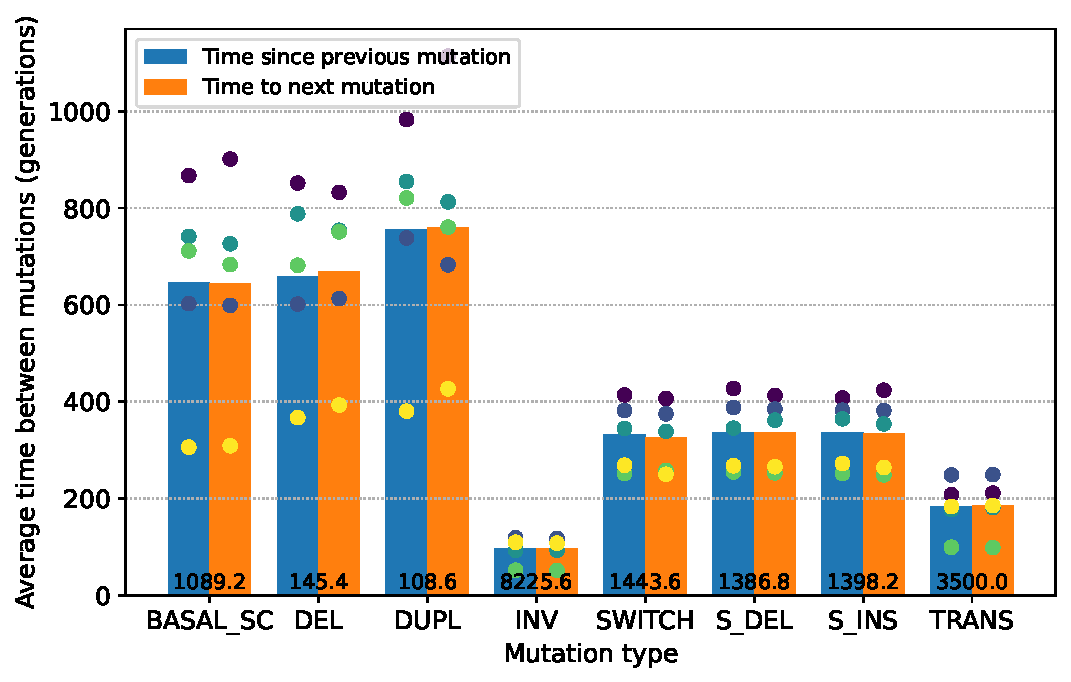
\includegraphics[width=\textwidth]{aevol/images/epistasis_sc.pdf}
  \end{subfigure}
  \begin{subfigure}[t]{\textwidth}
    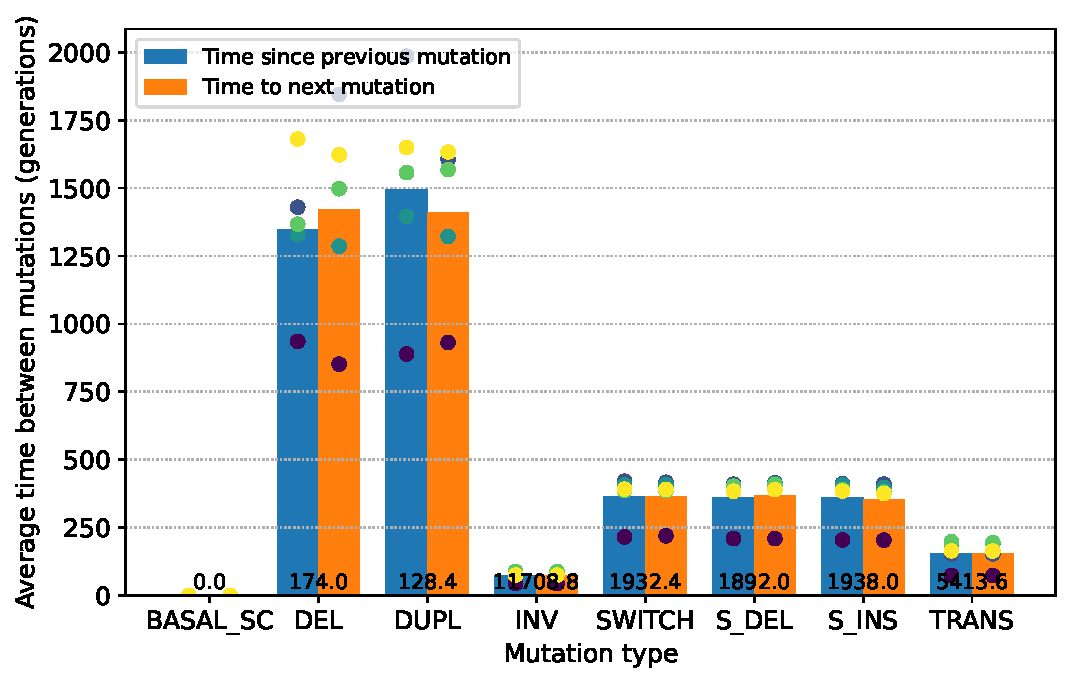
\includegraphics[width=\textwidth]{aevol/images/epistasis_control.pdf}
  \end{subfigure}
  \caption[Measuring epistasis with the average times before and after mutations]{Average time before and after a mutation of each kind, in the experimental runs (top) and the control runs (bottom).
  For each kind of mutation, the times presented show the wait time until a neutral mutation of that kind after a non-neutral mutation of any kind, and the time until the next non-neutral mutation of any kind after a mutation of that kind.
  The bars show the average over the five replicates, and the colored dots are the value for every replicate.
  The average number of neutral mutations of each type is displayed at the bottom of the corresponding bar.}
  \label{fig:aevol:epistasis}
\end{figure}

\paragraph{Role of the Genome Size}
A possible interpretation of the pattern visible in the control runs for the large deletions and duplications is that the difference in waiting times, and hence the positive or negative epistasis, is simply due to the change in the genome size caused by this mutations.
Indeed, all mutation rates are proportional to the genome size, and the number of mutations at each generation therefore increases and decreases with the genome size (assuming that there is no fitness effect or selection).
In the experimental runs, the probability of a supercoiling mutation importantly does not depend on the genome size, which could hide the epistasis signal between duplications or deletions and other mutation types.


\section{Conclusion}
\label{sec:aevol:ccl}

The goal of this initial work was to study the ways in which supercoiling mutations affect the fitness landscape, that is the possible epistatic interactions between supercoiling mutations and other kinds of mutations.
In order to approach this question, I implemented a model of the effect of the supercoiling level on gene expression, as well as a model of mutations in the supercoiling level, into the \emph{Aevol} \emph{in silico} experimental evolution platform.
I ran evolutionary experiments, in which I compared the evolution of populations using this model of supercoiling with control populations by analyzing the fitness, supercoiling level, and mutations fixed in the lineage of individuals that leads to the final population of every replicate.

With the limited data available, I could not find a difference in the evolution rates of each set of experiments, showing that supercoiling does not seem to play an important evolutionary role in this model; this result was substantiated by the fact that the supercoiling level converges very quickly to a fixed level in the evolutionary history of each population.
I then tried to detect signals of positive or negative epistasis between the different kinds of mutations, by looking at the waiting times between each kind of mutation.
While this approach did not lead to meaningful results in the experimental runs, it did hint at a possible epistatic link between duplications or deletions and the other mutation kinds, due to their effect on genome size, in the control runs.

\paragraph{}
The verdict of these preliminary experiments was that the model of supercoiling that I implemented in \emph{Aevol}, in which supercoiling is kept constant along the genome and affects the expression level of all genes equally, was probably too simplistic to obtain meaningful results as-is.
Rather than pursuing this avenue of research further by implementing a more precise model in \emph{Aevol}, I chose instead to go in a different direction.
In order to decouple the complexity of the \emph{Aevol} model from the study of the evolutionary role of supercoiling, I decided to simplify the individual model, genotype-phenotype map, and mutational operators as much as possible, in order to model the effect of supercoiling on gene expression more precisely while keeping the overall complexity of the model in check.
The results of this renewed approach are presented in the following chapters.